\chapter{Introduction}

\newpage
\section{Exercise 1-1}
The equation for the momentum
\begin{equation}
	p = \frac{h}{\lambda}
\end{equation}
has the following dimensions:
\[
	\left[\text{momentum}\right] = \frac{\left[\text{energy}\right] \left[\text{time}\right]}{\left[\text{length}\right]}
\]
The unit of energy is \si{\joule}, the unit of time is \si{\second}, and the
unit of length is \si{\meter}. Hence, we can perform the dimensional analysis
directly with the corresponding units which gives
\[
	p
	= \left[ \frac{\si{\joule} \si{\second}}{\si{\meter}} \right]
	= \left[ \frac{\si{\kilogram\meter\squared\second}}{\si{\second\squared\meter}} \right]
	= \left[ \frac{\si{\kilogram\meter}}{\si{\second}} \right]
\]

\newpage
\section{Exercise 1-2}
The workfunction $\phi$ of Titanium is
\[
	\phi
	= \SI{4.33}{\eV}
	= \SI{4.33}{\eV} \frac{\SI{1.6e-19}{\joule}}{\SI{1}{\eV}}
	= \SI{6.93e-19}{\joule}
\]
The work function $\phi$ describes the amount of energy that is required to
free an electron by incident EM radiation (i.e. light). Hence, this is the
absolute minimum required energy. Using the generic relation
$E - \phi = h f$ we thus get $E - \phi = 0$ and thus $E = \phi$. As we know
the energy and Planck's constant, we can solve for the frequency $f$
\[
	E = h f \quad \Rightarrow \quad f = \frac{E}{h}
\]
However, we are interested in the required frequency of the incident EM
radiation. Hence, we use the relation $c_0 = \lambda f$. With this we get
\[
	\lambda
	= \frac{c_0 h}{E}
	= \frac{\SI{3e8}{\meter\per\second} \cdot \SI{6.625e-34}{\joule\second}}{\SI{6.93e-19}{\joule}}
	= \SI{2.87e-7}{\meter}
\]

\lstinputlisting[caption=Exercise 1-2]{./../ch1/ex_1_2.m}

\newpage
\section{Exercise 1-3}
At the beginning, the electron is considered to have only KE and no PE. The
amount of initial KE ($KE_1$) can be calculated with the given initial
wavelength of $\lambda_1 = \SI{10}{\nano\meter}$. This gives us
\[
	KE_1
	= \frac{1}{2 m_e} \left(\frac{h}{\lambda_1}\right)^2
	= \frac{1}{2 \SI{9.11e-31}{\kg}} \left(\frac{\SI{6.625e-34}{\joule\second}}{\SI{10}{\nano\meter}}\right)^2
	= \SI{2.41e-21}{\joule}
\]
After going trough the potential of \SI{0.02}{\eV}, the electron gains
another \SI{0.02}{\eV} worth of KE. Hence, the resulting KE is
\[
	KE_2
	= KE_1 + \SI{0.02}{\eV}
	= \SI{2.41e-21}{\joule} + \SI{0.02}{\eV}\left(\frac{\SI{1.6e-9}{\joule}}{\SI{1}{\eV}}\right)
	= \SI{5.61}{\joule}
\]
Now that the resulting KE is known, the wavelength of the electron can be
determined as
\[
	\lambda
	= \frac{h}{\sqrt{2 KE_2 m_e}}
	= \frac{\SI{6.625e-34}{\joule\second}}{\sqrt{2 \SI{5.61}{\joule} \SI{9.11e-31}{\kg}}}
\]

\lstinputlisting[caption=Exercise 1-3]{./../ch1/ex_1_3.m}

\newpage
\section{Exercise 2-1}
As the particle goes into the barrier, a certain portion of its initial KE
is exchanged for PE. While the total energy stays the same, the wavelength
changes as it depends on the KE of the particle. As the particle has lower
KE, the wavelength gets larger (i.e. the frequency gets lower) according to
\[
	KE = \frac{1}{2 m_e} \left(\frac{h}{\lambda}\right)^2
	\Rightarrow
	\lambda = \frac{h}{\sqrt{2 KE m_e}}
\]

The imaginary part \emph{leads} the real part. This means that the direction
in which the wave propagates can be determined from the plot. The incident
wave prior to the particle arriving at the barrier, has a leading imaginary
part to the right. Hence, the particle is moving to the right and thus
towards the potential barrier. After the barrier is reached, the wave is
split in two parts; the incident wave is split in a transmissive and
reflective part. The transmissive part is the part right of the barrier, which
is in the direction of the incident wave. This is evident by the leading
imaginary part of the wave. However, the reflected part shows an imaginary
part which is to the left of the real part. Hence, this reflected part is
propagating in opposite direction of the incident wave.

\newpage
\section{Exercise 2-2}
In general, from an electrical engineers point of view, the Heisenberg
uncertainty principle describes the same relation as signals in the time and
frequency domain when performing the Fourier transforms. If a signal is very
localized in time (e.g. Dirac Delta function or step function), it's
bandwidth is very large (e.g. towards infinite bandwidth or white noise).
The same holds for the opposite direction. If a signal is very localized in
the frequency domain (i.e. a perfectly constant sine wave of frequency $f$),
the signal is very wide-spread in the time domain (i.e. starts in
$-\infty$ and goes until $+\infty$).

Figure 1.5 shows the wave of a particle which spreads out spatially about
\SI{20}{\nano\meter}. If we want to know the position of the particle
described by the shown wave in Figure 1.5, we can not perfectly localize
it. Hence, we have an uncertainty in position of the particle.

We can see that the center wavelenth is approximately \SI{10}{\nano\meter}.
However, the wave is not a simple sine wave consisting of a signle frequency
$f$. In fact, the shown waveform is a Gaussian envelop and this means that
the shown waveform consists of many different frequencies or wavelengths
around the center wavelength of \SI{10}{\nano\meter}. The momentum of the
particle is described by
\[
	p = \frac{h}{\lambda}
\]
If we want to know the exact momentum of the particle, we need an exact
value for its wavelength $\lambda$. However, herein lies the difficulty,
as we do not knwo the exact wavelength of the particle and hence we
have an uncertainty in the particles momentum.

In Figure 1.5 we see a typical example of a particle, that is we have an
uncertainty in both position and momentum. However, it would be good to
imagine the two extreme cases where the uncertainty of either the momentum
or the position is going towards zero.

\newpage
\section{Exercise 2-3}

\subsection{1-D Case}
To derive the unit of the 1-D wavefunction $\psi(x)$ we can analyze the
normalized probability calculation for the position
\[
	\braket{\psi(x)|\psi(x)}
	= \int_{-\infty}^{+\infty}{\abs{\psi(x)}^2} \dif x
	= 1
\]
The physical interpretation of this equation is that the square of the 
wavefunction gives the probability(density) to find the particle in a
region of \emph{distance} $x$. If we integrate this along $x$, we get
the probability that the particle is within the investigated region of $x$.

In this equation we see that we integrate over distance ($\dif x$). Hence,
the integration gives a dimension of length [L]. As the result is $1$,
which is dimensionless, the integrand must be of the inverse
unit, i.e. $[L^{-1}]$. The integrand is the square of the wavefunction
$\abs{\psi(x)}^2$. Therefore, the wavefunction itself must have the unit of
$[\sqrt{L^{-1}}]$ or $[L^{\frac{-1}{2}}]$.

\subsection{2-D Case}
In the 2-D case, we no longer investigate a simple distance but a \emph{surface}.
Thus, instead of $\int \dif x$ we now use $\int \dif s$. Analogous to the
1-D case, we can identify that the integration gives a dimension of $[L^2]$.
To get a dimensionless result, the square of the wavefunction
$\abs{\psi(x,y)}^2$ must have the unit of $[L^{-2}]$. Therefore, the
wavefunction itself must have the unit of $[\sqrt{L^{-2}}]$ or $[L^{-1}]$.

\subsection{3-D Case}
Analogous to the 2-D case, for the 3-D case we investigate a \emph{volume}.
Hence, we now use $\int \dif V$. The integration thus gives a dimension of
$[L^3]$. To get a dimensionless result, the square of the wavefunction
$\abs{\psi(x,y,z)}^2$ must have the unit of $[L^{\frac{-3}{2}}]$.

% \begin{table}[h!]
% 	\centering
% 	\caption{Dimension and units of the wavefunction}
% 	\begin{tabular}{l c c}
% 		\toprule
% 		dimension 	& dimension of $\psi$	& unit				\\
% 		\midrule
% 		\bottomrule
% 	\end{tabular}
% \end{table}

\newpage
\section{Exercise 2-4}
The probability that the particle is located in a region $a \leq x \leq b$ is
given by the integral of the squared wavefunction $\abs{\psi(x)}^2$ over that
region. Hence, the square of the wavefunction is the probability density.
However, we must not forget to apply normalization, which is performed by
setting the integral over the total region equal to 1. If not specified
otherwise, this is in general $-\infty \leq x \leq +\infty$.

In Figure 1.13 a complex waveform is shown. As stated in the hint to the
exercise, we can approximate the magnitude (i.e. amplitude) of the shown
wave picewise for the different regions. First, we assume that the magnitude
is zero for $x \leq \SI{5}{\nano\m}$ and $x \geq \SI{30}{\nano\m}$. Next,
we define the amplitudes with a common variable $A$, which is the maximum
magnitude. Every other value of the magnitude is expressed relative to $A$
as $kA$. The approximation made is shown in Figure \ref{fig:ex_2_4_magnitude}.

\begin{figure}[h!]
	\centering
	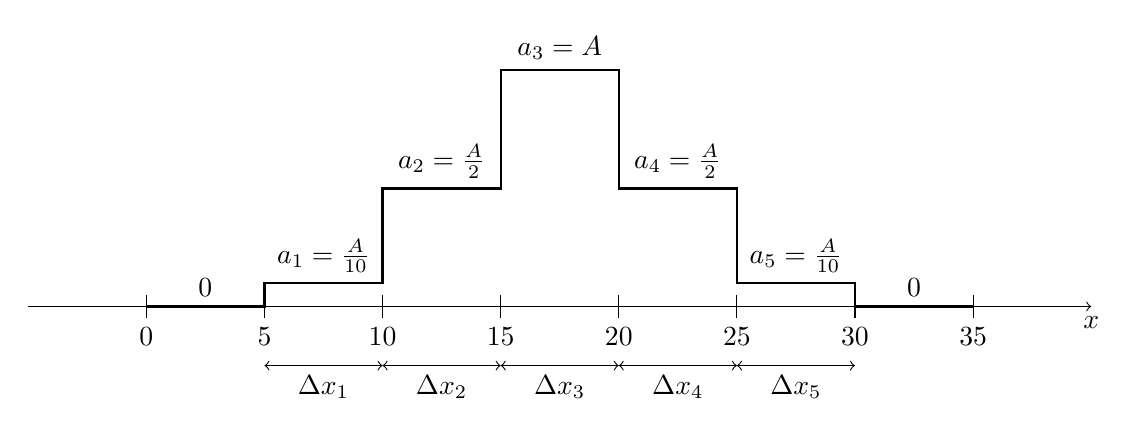
\begin{tikzpicture}[scale=1.5]
		\def\A{2}
		\def\tk{0.1}
		\draw[->] (-1,0) -- (8,0) node (xaxis) [below] {$x$};
		% draw the picewise linear magnitude
		\draw[thick]
			(0, 0.0 * \A) -- node [above] {$0$}
			(1, 0.0 * \A) --
			(1, 0.1 * \A) -- node [above] {$a_1=\frac{A}{10}$}
			(2, 0.1 * \A) --
			(2, 0.5 * \A) -- node [above] {$a_2=\frac{A}{2}$}
			(3, 0.5 * \A) --
			(3, 1.0 * \A) -- node [above] {$a_3=A$}
			(4, 1.0 * \A) --
			(4, 0.5 * \A) -- node [above] {$a_4=\frac{A}{2}$}
			(5, 0.5 * \A) --
			(5, 0.1 * \A) -- node [above] {$a_5=\frac{A}{10}$}
			(6, 0.1 * \A) --
			(6, 0.0 * \A) -- node [above] {$0$}
			(7, 0.0 * \A);
		% mark ticks
		\draw (0, \tk) -- (0, -\tk) node [below] {$\SI{0}{\nano\m}$};
		\draw (1, \tk) -- (1, -\tk) node [below] {$\SI{5}{\nano\m}$};
		\draw (2, \tk) -- (2, -\tk) node [below] {$\SI{10}{\nano\m}$};
		\draw (3, \tk) -- (3, -\tk) node [below] {$\SI{15}{\nano\m}$};
		\draw (4, \tk) -- (4, -\tk) node [below] {$\SI{20}{\nano\m}$};
		\draw (5, \tk) -- (5, -\tk) node [below] {$\SI{25}{\nano\m}$};
		\draw (6, \tk) -- (6, -\tk) node [below] {$\SI{30}{\nano\m}$};
		\draw (7, \tk) -- (7, -\tk) node [below] {$\SI{35}{\nano\m}$};
		% draw intervals
		\draw[<->] (1, -5*\tk) -- node [below] {$\Delta x_1$} (2, -5*\tk);
		\draw[<->] (2, -5*\tk) -- node [below] {$\Delta x_2$} (3, -5*\tk);
		\draw[<->] (3, -5*\tk) -- node [below] {$\Delta x_3$} (4, -5*\tk);
		\draw[<->] (4, -5*\tk) -- node [below] {$\Delta x_4$} (5, -5*\tk);
		\draw[<->] (5, -5*\tk) -- node [below] {$\Delta x_5$} (6, -5*\tk);
	\end{tikzpicture}
	\caption{Piecewise approximated magnitude of the wavefunction.}
	\label{fig:ex_2_4_magnitude}
\end{figure}

From Figure \ref{fig:ex_2_4_magnitude} we see that the factor are
$k_3 = 1$, $k_4=k_2=\frac{1}{2}$, and $k_5=k_1=\frac{1}{10}$.
As we now do not have a continuous function over $x$ but a piecewise
constant over equidistant intervals (i.e. discrete in amplitude and $x$),
we can replace the continuous integration with a simple sum.
\[
	\int_a^b \abs{\psi(x)}^2 \dif x = 1
	\quad \rightarrow \quad
	\sum_{i=1}^{N} {a_i}^2 \Delta x_i = 1
\]
As we omit all zero-valued intervals, only five intervals are left where two
of them are the same due to symmetry, as shown in Figure
\ref{fig:ex_2_4_magnitude}.
\[
	{a_1}^2 \Delta x_1 + {a_2}^2 \Delta x_2 + {a_3}^2 \Delta x_3 + {a_4}^2 \Delta x_4 + {a_5}^2 \Delta x_5 = 1
\]
As $a_1 = a_5$ and $a_2 = a_4$, we can reduce the equation to
\[
	{a_3}^2 \Delta x_3 + 2 \left({a_4}^2 \Delta x_4\right) + 2 \left({a_5}^2 \Delta x_5\right) = 1
\]
If we insert the magnitudes for $a_i$ we get
\[
	\left(k_3A\right)^2 \Delta x_1 + 2 \left(k_4A\right)^2 \Delta x_2 + 2 \left(k_5A\right)^2 \Delta x_3 = 1
\]
As the intevals are all the same with
\[
	\Delta x_1
	= \SI{10}{\nano\m} - \SI{5}{\nano\m}
	= \SI{5}{\nano\m}
	= \Delta x_2 = \dots = \Delta x_5
	\quad \Rightarrow \quad 
	\Delta x = \Delta x_1 = \dots = \Delta x_5
\]
we can simplify by factorization and get
\[
	\Delta x \left( \left(k_3A\right)^2 + 2 \left(k_4A\right)^2 + 2 \left(k_5A\right)^2 \right) = 1
\]
To solve for the probabilities $p_i$, we now need to solve for $A^2$, which is
\[
	A^2 = \frac{1}{\Delta x \left(k_3^2 + 2 k_4^2 + 2 k_5^2\right)}
\]
Knowing the value of $A^2$ allows us to calculate the probabilities for the
individual intervals.
\[
	p_i = {k_i}^2 A^2 \Delta x_i
\]
\[
	\begin{bmatrix}
		p_3 \\
		p_4 \\
		p_5 \\
	\end{bmatrix}
	=
	\begin{bmatrix}
		0.658 \\
		0.164 \\
		0.007 \\
	\end{bmatrix}	
\]


\lstinputlisting[caption=Exercise 2-4]{./../ch1/ex_2_4.m}

\newpage
\section{Exercise 2-5}

Figures \ref{fig:ex_2_5_a} and \ref{fig:ex_2_5_b} show the simulation results
for the wave with different wavelengts ($\lambda_1 = \SI{10}{\nano\m}$,
$\lambda_2 = \SI{20}{\nano\m}$). The results show that the wave with the
shorter wavelength is propagating faster. The reason for this is simple, the
shorter the wavelength the higher the KE and hence the higher the velocity.

Figure \ref{fig:ex_2_5_c} shows the simulation result for the negative
wavelength ($\lambda = \SI{-10}{\nano\m}$). Using a negative wavelenght the
direction in which the wave propagates changes. Hence, the wave is now
propagating to the left (negative to $x$). Again, the imaginary part is leading.
Besides the direction, everything else stays the same as compared to a
positive wavelength.

\newpage

\begin{figure}
	\centering
	\begin{subfigure}{1\linewidth}
		\includegraphics[width=1\linewidth]{./../ch1/ex_2_5_a_0.png}
	\end{subfigure}

	\begin{subfigure}{1\linewidth}
		\includegraphics[width=1\linewidth]{./../ch1/ex_2_5_a_1.png}
	\end{subfigure}
	
	\begin{subfigure}{1\linewidth}
		\includegraphics[width=1\linewidth]{./../ch1/ex_2_5_a_2.png}
	\end{subfigure}
	
	\caption{$\lambda = \SI{10}{\nano\m}$.}
	\label{fig:ex_2_5_a}
\end{figure}

\newpage

\begin{figure}
	\centering
	\begin{subfigure}{1\linewidth}
		\includegraphics[width=1\linewidth]{./../ch1/ex_2_5_b_0.png}
	\end{subfigure}

	\begin{subfigure}{1\linewidth}
		\includegraphics[width=1\linewidth]{./../ch1/ex_2_5_b_1.png}
	\end{subfigure}
	
	\begin{subfigure}{1\linewidth}
		\includegraphics[width=1\linewidth]{./../ch1/ex_2_5_b_2.png}
	\end{subfigure}
	
	\caption{$\lambda = \SI{20}{\nano\m}$.}
	\label{fig:ex_2_5_b}
\end{figure}

\newpage

\begin{figure}
	\centering
	\begin{subfigure}{1\linewidth}
		\includegraphics[width=1\linewidth]{./../ch1/ex_2_5_c_0.png}
	\end{subfigure}

	\begin{subfigure}{1\linewidth}
		\includegraphics[width=1\linewidth]{./../ch1/ex_2_5_c_1.png}
	\end{subfigure}
	
	\begin{subfigure}{1\linewidth}
		\includegraphics[width=1\linewidth]{./../ch1/ex_2_5_c_2.png}
	\end{subfigure}
	
	\caption{$\lambda = \SI{-10}{\nano\m}$.}
	\label{fig:ex_2_5_c}
\end{figure}

\clearpage

\lstinputlisting[caption=Exercise 2-5 a]{./../ch1/ex_2_5_a.m}
\lstinputlisting[caption=Exercise 2-5 b]{./../ch1/ex_2_5_b.m}
\lstinputlisting[caption=Exercise 2-5 c]{./../ch1/ex_2_5_c.m}

\subsection{Discussion on Code Efficiency}
The author's code uses a lot of loops to manipulate the values of the vector
data. While this is the common way to do it in most programming languages,
MATLAB and GNU Octave have very specific features to implement such operations
not just more elegantly in syntax but can also boost performance of the code
substantially. I have introduced wherever possible such alternative
implementations but left the original loop code as commented section available
to the reader.

The performance difference was evaluated using the code for exercise 2-5 with
the following results.

\begin{table}[h!]
	\centering
	\caption{Performance comparison of loops vs. matrix operations.}
	\begin{tabular}{l c}
		\hline
		variant			& time									\\
		\hline
		FDTD using for loops 			& \SI{8.17}{\second} 	\\
		FDTD using matrix operations 	& \SI{1.80}{\second}	\\
		\hline
	\end{tabular}
\end{table}


\newpage
\section{Exercise 3-1}

\subsection{Expectation Value}

The expectation value of the position $\braket{x}$ is defined as
\[
	\braket{x} = \int_{-\infty}^{\infty} \varPsi^{\ast}(x) x \varPsi(x) \dif x
\]
To calculate $\braket{x}$ in the FDTD format, we can use
\begin{align*}
	\braket{x} &= \sum_{n=1}^{NN} \left[ \varPsi_{real}(n) - i \varPsi_{imag}(n) \right] (n \cdot \Delta x) \left[ \varPsi_{real}(n) + i \varPsi_{imag}(n) \right] \\
	&= \sum_{n=1}^{NN} \left[ \varPsi^2_{real}(n) + \varPsi^2_{imag}(n) \right] (n \cdot \Delta x)
\end{align*}
This can easily be implemented and added to the existing code, which produces
the plots showed in Figure \ref{fig:ex_3_1_a}.

\begin{figure}
	\centering
	\begin{subfigure}{1\linewidth}
		\includegraphics[width=1\linewidth]{./../ch1/ex_3_1_a_0.png}
	\end{subfigure}
	
	\begin{subfigure}{1\linewidth}
		\includegraphics[width=1\linewidth]{./../ch1/ex_3_1_a_1.png}
	\end{subfigure}
	
	\begin{subfigure}{1\linewidth}
		\includegraphics[width=1\linewidth]{./../ch1/ex_3_1_a_2.png}
	\end{subfigure}
	
	\caption{$\lambda = \SI{20}{\nano\m}$.}
	\label{fig:ex_3_1_a}
\end{figure}

\clearpage

\lstinputlisting[caption=Exercise 3-1 a]{./../ch1/ex_3_1_a.m}

\subsection{Expectation Value with Barrier}

The expectation value $\braket{x}$ is an average scalar value.
If the particle hits a potential barrier, there is a transmissive
and reflective part propagating in opposite directions, i.e. the
particle is split, see Figure \ref{fig:ex_3_1_b}. Hence, an average
position can be calculated, however, it does not really make sense.

\begin{figure}
	\centering
	\begin{subfigure}{1\linewidth}
		\includegraphics[width=1\linewidth]{./../ch1/ex_3_1_b_0.png}
	\end{subfigure}
	
	\begin{subfigure}{1\linewidth}
		\includegraphics[width=1\linewidth]{./../ch1/ex_3_1_b_1.png}
	\end{subfigure}
	
	\begin{subfigure}{1\linewidth}
		\includegraphics[width=1\linewidth]{./../ch1/ex_3_1_b_2.png}
	\end{subfigure}
	
	\caption{$\lambda = \SI{20}{\nano\m}$.}
	\label{fig:ex_3_1_b}
\end{figure}

\clearpage

\lstinputlisting[caption=Exercise 3-1 b]{./../ch1/ex_3_1_b.m}

\newpage
\section{Exercise 4-1}

The electric field strength $E$ needs to be converted into a potential $V$
using the given path length $s$. 
\[
	V = E s
	  = \SI{5e6}{\volt\per\meter} \SI{40e-9}{\meter}
	  = \SI{0.2}{\volt}
\]
The problem does not specify exactly how the potential is laid out,
however, the solution implies that we should place it such that the
potential is symmetric starting at $p$ and going to $-p$. Hence,
we start at \SI{0.1}{\volt} and end at \SI{-0.1}{\volt}.

The simulation results show that the particle looses potential energy
and gains kinetic energy while moving to the right. So, the particle
\emph{trades} potential energy for kinetic energy as it moves along
the potential.

\begin{figure}
	\centering
	\begin{subfigure}{1\linewidth}
		\includegraphics[width=1\linewidth]{./../ch1/ex_4_1_0.png}
	\end{subfigure}
	
	\begin{subfigure}{1\linewidth}
		\includegraphics[width=1\linewidth]{./../ch1/ex_4_1_1.png}
	\end{subfigure}
	
	\begin{subfigure}{1\linewidth}
		\includegraphics[width=1\linewidth]{./../ch1/ex_4_1_2.png}
	\end{subfigure}
	
	\caption{$\lambda = \SI{40}{\nano\m}$.}
	\label{fig:ex_4_1}
\end{figure}

\clearpage

\lstinputlisting[caption=Exercise 4-1]{./../ch1/ex_4_1.m}

\newpage
\section{Exercise 4-2}

\begin{figure}
	\centering
	\begin{subfigure}{1\linewidth}
		\includegraphics[width=1\linewidth]{./../ch1/ex_4_2_0.png}
	\end{subfigure}
	
	\begin{subfigure}{1\linewidth}
		\includegraphics[width=1\linewidth]{./../ch1/ex_4_2_1.png}
	\end{subfigure}
	
	\begin{subfigure}{1\linewidth}
		\includegraphics[width=1\linewidth]{./../ch1/ex_4_2_2.png}
	\end{subfigure}
	
	\caption{$\lambda = \SI{40}{\nano\m}$.}
	\label{fig:ex_4_2}
\end{figure}

\clearpage

\lstinputlisting[caption=Exercise 4-2]{./../ch1/ex_4_2.m}

\newpage
\section{Exercise 5-1}

The simulation shows an initial amplitude of approx. \SI{0.15}{\eV}. After
the barrier, we see the transmitted wave with an amplitude of
$a_t \approx \SI{0.03}{\eV}$ and the reflected wave with an amplitude of
$a_r \approx \SI{0.1}{\eV}$. For simplicity, we can say that the amplitude
of the reflected wave is three times higher than the transmitted wave with
$a_r = 3 a_t$.
%
The probability of a particle being in a specified region of $x$ is
determined by
%
\[
	P = \int_{x_1}^{x_2} \abs{\varPsi(x)}^2 \dif x
\]
%
The exact solution would be to calculate the probability with the above
integral for both regions, i.e. left of the barrier for the reflected and
right of the barrier for the transmitted wave. A simple estimation can be
found by just using the amplitude $a$ with $P = \int_{x} a^2 \dif x$. Using
this simplification, the probability can be expressed as $P = a^2 \Delta x$,
which gives us
\begin{align*}
	P_t &= {a_t}^2 \Delta x_t \\
	P_r &= {a_r}^2 \Delta x_r
\end{align*}
Since we are interested in the relative probability that the particle passed
the barrier, we can express is as
\[
	P
	= \frac{P_t}{P_t + P_r}
	= \frac{{a_t}^2 \Delta x_t}{{a_t}^2 \Delta x_t + {a_r}^2 \Delta x_r}
\]
Assuming that the range for both sides is approximately equal with
$x_t \approx x_r$, we can further simplify to
\[
	P
	= \frac{P_t}{P_t + P_r}
	= \frac{{a_t}^2 \Delta x}{({a_t}^2 + {a_r}^2) \Delta x}
	= \frac{{a_t}^2}{{a_t}^2 + {a_r}^2}
\]
Using the relative amplitudes with $a_r = 3 a_t$, the relative probability
that the particle passed the barrier is
\[
	P
	= \frac{P_t}{P_t + P_r}
	= \frac{{a_t}^2}{{a_t}^2 + {a_r}^2}
	= \frac{{a_t}^2}{{a_t}^2 + (3 a_t)^2}
	= \frac{{a_t}^2}{{a_t}^2 + 9 {a_t}^2}
	= \frac{{a_t}^2}{10 {a_t}^2}
	= \frac{1}{10}
	= 0.1 \\
\]
Using the same approach, we can determine the probability for the particle
being reflected to be
\[
	P
	= \frac{P_r}{P_t + P_r}
	= \frac{{a_r}^2}{{a_t}^2 + {a_r}^2}
	= \frac{(3 a_t)^2}{{a_t}^2 + (3 a_t)^2}
	= \frac{9 {a_t}^2}{{a_t}^2 + 9 {a_t}^2}
	= \frac{9 {a_t}^2}{10 {a_t}^2}
	= \frac{9}{10}
	= 0.9 \\
\]
So, the probability of the particle passing the barrier is \SI{10}{\percent}
and the probability of the particle being reflected is \SI{90}{\percent}.

\newpage
\section{Generating GIF}
Instead of just generating a series of individual images, a GIF can also
be generated using GNU Octave. The FDTD script used in the previous exercises
was modified such that a GIF is generated.

\lstinputlisting[caption=Experiment 2 - GIF]{./../ch1/experiment_2_gif.m}